%-----------------------------------------------------------------------------------------------%
%
% Maret 2019
% Template Latex untuk Tugas Akhir Program Studi Sistem informasi ini
% dikembangkan oleh Inggih Permana (inggihjava@gmail.com)
%
% Template ini dikembangkan dari template yang dibuat oleh Andreas Febrian (Fasilkom UI 2003).
%
% Orang yang cerdas adalah orang yang paling banyak mengingat kematian.
%
%-----------------------------------------------------------------------------------------------%

%-----------------------------------------------------------------------------%
\chapter{\babDua}
%-----------------------------------------------------------------------------%
Tidak ada batasan membuat subbab pada Bab 2. Buatlah subbab sesuai kebutuhan tugas akhir anda.


%-----------------------------------------------------------------------------%
\section{Bagaimana Cara membuat tulisan Bold, Italic, dan Underline?}
%-----------------------------------------------------------------------------%
Berikut cara membuat tulisan \textbf{bold}, \textit{italic}, dan \underline{underline} ini dia: 

\begin{enumerate}
	\item \textbf{Bold}: Gunakan perintah \bslash textbf$\lbrace\rbrace$.
	\item \textit{Italic}: Gunakan perintah \bslash textit$\lbrace\rbrace$.
	\item \underline{Underline}: Gunakan perintah \bslash underline$\lbrace\rbrace$.
\end{enumerate}

%-----------------------------------------------------------------------------%
\section{Bagaimana Cara membuat tulisan $^{superscript}$ dan $_{subscript}$?}
%-----------------------------------------------------------------------------%
Berikut cara membuat tulisan \textbf{bold}, \textit{italic}, dan \underline{underline} ini dia: 

\begin{enumerate}
	\item $^{superscript}$: Gunakan perintah \$ $\wedge$ $\lbrace\rbrace$ \$. 
	\item $_{subscript}$: Gunakan perintah \$ \_$\lbrace\rbrace$ \$. 
\end{enumerate}

%-----------------------------------------------------------------------------%
\section{Bagaimana Cara Memasukkan Gambar?}
%-----------------------------------------------------------------------------%
Cara memasukkan gambar di latex dapat dilihat pada \pic~\ref{gambarA}. Hasil dari kompilasi \pic~\ref{gambarA} dapat dilihat pada \pic~\ref{gambarA}. Contoh gambar yang ada referensinya dapat dilihat pada \pic~\ref{gambarB}.

\begin{figure}
	\centering
	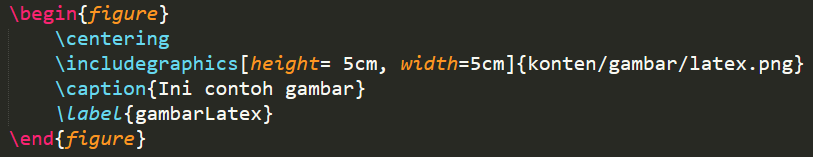
\includegraphics[height= 3cm, width=10.5cm]{konten/gambar/contohGambar.png}
	\caption{Cara memasukkan gambar di Latex}
	\label{gambarA}
\end{figure}

\begin{figure}
	\centering
	
\includegraphics[height= 5cm, width=5cm]{konten/gambar/latex.png}
	\caption{Latex itu sederhana \protect\cite{arfajsyah2018sistem}}
	\label{gambarB}
\end{figure}


Berikut hal-hal yang perlu diketahui dalam memasukkan gambar di Latex: 

\begin{enumerate}
	\item Setiap gambar harus diberikan caption dan diberikan label. 
	\item Label dapat digunakan untuk merujuk gambar tertentu dengan kode \bslash pic $\backsim$ \bslash ref $\lbrace namaLabel \rbrace$.
	\item Jika posisi gambar berubah, maka nomor gambar juga akan diubah secara 
otomatis. Begitu juga dengan seluruh kalimat yang merujuk pada gambar tersebut.
\end{enumerate}

%-----------------------------------------------------------------------------%
\section{Bagaimana Cara Membuat Tabel}
%-----------------------------------------------------------------------------%
Seperti pada gambar, tabel juga dapat diberi label dan caption. Caption pada tabel terletak pada bagian atas tabel. Contoh tabel sederhana dapat dilihat pada \tab~\ref{tabelA}. Contoh tabel dengan penggabungan baris dan penggabungan kolom dapat dilihat pada \tab~\ref{tabelB}. Contoh tabel dengan tulisan vertikal dapat dilihat pada \tab~\ref{tabelC}. Contoh tabel skenario dapat dilihat pada \tab~\ref{tabelD}. Contoh tabel \textit{landscape} dapat dilihat pada \tab~\ref{tabelE}. Contoh tabel yang ada referensinya dapat dilihat pada \tab~\ref{tabelB}.

%======================================================================%
{
\fontsize{10}{12}\selectfont
\begin{longtable}{p{3cm} p{3cm} p{3cm}}
	\caption{Contoh tabel pertama}\\
	\hline
	\textbf{Variabel A} & \textbf{Variabel B} & \textbf{Variabel C}\\
	\hline
	\endfirsthead

	\multicolumn{3}{c}{\tablename\ \thetable\ Contoh tabel pertama \space (Tabel lanjutan...)} \\
	\hline
	\textbf{Variabel A} & \textbf{Variabel B} & \textbf{Variabel C}\\
	\hline
	\endhead

	A & B & C\\
	D & E & F\\
	G & H & I\\
	J & K & L\\ \hline

\label{tabelA}
\end{longtable}
}

%=====================================================================%
{
\fontsize{10}{12}\selectfont
\begin{longtable}{p{3cm} p{4cm} p{3cm}}
	\caption{Gabung baris/kolom pada tabel \protect\cite{sari2017sistem}}\\
	\hline
	\textbf{No. Transaksi} & \textbf{Item} & \textbf{Qty}\\
	\hline
	\endfirsthead

	\multicolumn{3}{c}{\tablename\ \thetable\ Gabung baris/kolom pada tabel \protect\cite{sari2017sistem} \space (Tabel lanjutan...)} \\
	\hline
	\textbf{No. Transaksi} & \textbf{Item} & \textbf{Qty}\\
	\hline
	\endhead

	\multirow{2}{\linewidth}{1} & Mie Rebus Instan & 3\\
	 & Mie Goreng Instan & 1\\
	\multirow{3}{\linewidth}{2} & Air Mineral & 4\\
	 & Roti Coklat & 5\\
	 & Gula & 3\\
	 \hline
	\multicolumn{2}{p{7cm}}{Jumlah} & 16\\ \hline

\label{tabelB}
\end{longtable}
}


%============================================================================%
{
\fontsize{10}{12}\selectfont
\begin{longtable}{p{0.5cm} p{0.5cm} p{0.5cm} p{0.5cm} p{0.5cm} p{0.5cm} p{0.5cm} p{0.5cm} p{0.5cm} p{0.5cm}}
	\caption{Contoh tulisan vertikal pada tabel}\\
	\hline
	\textbf{No.} & \rotatebox{90}{\textbf{Item 1}} & \rotatebox{90}{\textbf{Item 2}} & \rotatebox{90}{\textbf{Item 3}} & \rotatebox{90}{\textbf{Item 4}} & \rotatebox{90}{\textbf{Item 5}} & \rotatebox{90}{\textbf{Item 6}} & \rotatebox{90}{\textbf{Item 7}} & \rotatebox{90}{\textbf{Item 8}} & \rotatebox{90}{\textbf{Item 9}}\\
	\hline
	\endfirsthead

	\multicolumn{10}{c}{\tablename\ \thetable\ Contoh tulisan vertikal pada tabel \space (Tabel lanjutan...)} \\
	\hline
	\textbf{No.} & \rotatebox{90}{\textbf{Item 1}} & \rotatebox{90}{\textbf{Item 2}} & \rotatebox{90}{\textbf{Item 3}} & \rotatebox{90}{\textbf{Item 4}} & \rotatebox{90}{\textbf{Item 5}} & \rotatebox{90}{\textbf{Item 6}} & \rotatebox{90}{\textbf{Item 7}} & \rotatebox{90}{\textbf{Item 8}} & \rotatebox{90}{\textbf{Item 9}}\\
	\hline
	\endhead

	1 & 1 & 1 & 0 & 0 & 0 & 0 & 0 & 0 & 0\\
	2 & 0 & 0 & 0 & 1 & 1 & 0 & 0 & 0 & 0\\
	3 & 0 & 0 & 0 & 0 & 0 & 0 & 0 & 1 & 1\\ \hline

\label{tabelC}
\end{longtable}
}

%=============================================================================%

{
\fontsize{10}{12}\selectfont
\begin{longtable}{p{6.5cm} p{6.5cm}}

	\caption{Contoh tabel skenario}\\
	\hline
	\multicolumn{2}{p{13cm}}{\textbf{Nama Use Case:} Disini isi nama usecase anda}\\
	\multicolumn{2}{p{13cm}}{\textbf{Deskripsi:} Disini isi deksripsi usecase anda}\\
	\multicolumn{2}{p{13cm}}{\textbf{Tujuan:} Disini isi tujuan usecase anda}\\
	\multicolumn{2}{p{13cm}}{\textbf{Aktor:} Disini isi aktor yang terlibat}\\
	\multicolumn{2}{p{13cm}}{\textbf{Kondisi Awal:} Disini isi kondisi awal}\\
	\multicolumn{2}{p{13cm}}{\textbf{Kondisi Akhir:} Disini isi kondisi akhir}\\
	\hline
	\endfirsthead

	\multicolumn{2}{c}{\tablename\ \thetable\ Contoh tabel skenario \space (Tabel lanjutan...)} \\
	\hline
	\multicolumn{2}{p{13cm}}{\textbf{Nama Use Case:} Disini isi nama usecase anda}\\
	\multicolumn{2}{p{13cm}}{\textbf{Deskripsi:} Disini isi deksripsi usecase anda}\\
	\multicolumn{2}{p{13cm}}{\textbf{Tujuan:} Disini isi tujuan usecase anda}\\
	\multicolumn{2}{p{13cm}}{\textbf{Aktor:} Disini isi aktor yang terlibat}\\
	\multicolumn{2}{p{13cm}}{\textbf{Kondisi Awal:} Disini isi kondisi awal}\\
	\multicolumn{2}{p{13cm}}{\textbf{Kondisi Akhir:} Disini isi kondisi akhir}\\
	\hline
	\endhead


	\multicolumn{2}{c}{\textbf{Skenario Normal}}\\ \hline
	\multicolumn{1}{c}{\textbf{Aksi Aktor}} & \multicolumn{1}{c}{\textbf{Aksi Sistem}}\\
	1. Aksi normal 1 & \\
	2. Aksi normal 2 &\\
	& 3. Aksi normal 3\\
	& 4. Aksi normal 4\\

	\hline
	\multicolumn{2}{c}{\textbf{Skenario Gagal}}\\ \hline
	\multicolumn{1}{c}{\textbf{Aksi Aktor}} & \multicolumn{1}{c}{\textbf{Aksi Sistem}}\\
	1. Aksi gagal 1 & \\
	2. Aksi gagal 2 &\\
	& 3. Aksi gagal 3\\
	& 4. Aksi gagal 4\\ \hline

\label{tabelD}
\end{longtable}
}

%=================================================================%
{
\fontsize{10}{12}\selectfont
\begin{landscape}
\begin{longtable}[c]{llll}
\caption{Contoh tabel landscape}
\label{tabelE}\\
\hline
\textbf{Variabel A} & \textbf{Variabel B} & \textbf{Variabel C} & \textbf{Variabel D} \\ \hline
\endfirsthead
%
\multicolumn{4}{c}%
{{\bfseries \tablename\ \thetable\ Contoh tabel landscape}} \\
\hline
\textbf{Variabel A} & \textbf{Variabel B} & \textbf{Variabel C} & \textbf{Variabel D} \\ \hline
\endhead
%
\multirow{2}{*}{A} & B & C & D \\
 & F & G & H \\
I & J & K & L \\ \hline
\end{longtable}
\end{landscape}
}

